\chapter{PCA}
\label{section:pca}


In this chapter we explain the derivation of PCA and the algorithm for compressing and decompressing the BTF.
We have chosen PCA for BTF compression, which belong to statistical methods, see Chapter \ref{section:stat_methods}.
PCA compression method allows for easy regulation of trade-off between rendering quality and compression ratio.
While probabilistic methods have better compression ratio they are generally suited for flat materials \cite{haindl}.
Analytical methods can produce errors at gazing angles and generally have bigger decompression error than PCA \cite{haindl}.
Also, the PCA is suitable for the streaming very well, because the components are sorted in the order of the importance.
This means there is no need to do additional analysis to decide in which order to send the components.
Based on the above reasons, we chose PCA over other methods.


 \section{Derivation of PCA}
\label{section:derivation_pca}

 PCA can be defined through a maximum variance formulation, as done by Bishop \cite{Bishop}.
 Consider a set of variables $\left \{ x_{n} \right \}$, where $n=1..N$. $x_{n}$ are D-dimensional vectors. The goal is to project this data to an orthogonal basis while maximizing the variation of each new variable.
For the sake of simplicity, consider the projection to a one-dimensional space, i.e. to a new basis which consist of one vector $u_{1}$. 
As the magnitude of the vector is not important in this case, let it be a unit vector, i.e. $u_{1}^Tu_{1}=1$.
 Then, each variable $x_{n}$ is projected onto the new basis, i.e. a scalar $u_{1}^Tx_{n}$.

 To compute the variance of the projected data, first we need to define the mean of projected data:

{\centering$\tfrac{1}{N}\sum_{n=1}^{N}u_{1}^Tx_{n}=u_{1}^T(\tfrac{1}{N}\sum_{n=1}^{N}x_{n})=u_{1}^T\overline{x}.$\\}

Then, the variance of the projected data can be expressed:

{\centering$\sum_{n=1}^{N}(u_{1}^Tx_{n}-u_{1}^T\overline{x} )^2=u_{1}^TSu_{1}$\\}

where $S$ is the covariance matrix defined as:

{\centering$S=\sum_{n=1}^{N}(x_{n}-\overline{x})(x_{n}-\overline{x})^T.$\\}

The next step is to maximize the variance $u_{1}^TSu_{1}$ with respect to $u_{1}$. In order to avoid $\left \| u_{1} \right \|$ growing to infinity, additional constrain has to be used,
i.e.  normalization constrain $u_{1}^Tu_{1}=1$.

Then, the problem can be expressed as an optimization problem:

{\centering$maximize\,\,\,\,\,\,u_{1}^TSu_{1}$\\}

{\centering$\,\,\,\,\,subject \,\,to \,\,\,\,\,\,u_{1}^Tu_{1}=1$\\}

This can be solved with a Lagrangian multiplier:

{\centering$u_{1}^TSu_{1}+\lambda_{1}(1-u_{1}^Tu_{1}).$\\}

By taking the derivative with respect to $u_{1}$ and setting it to zero, the local extremum can be found:

{\centering$\frac{\partial }{\partial u_{1}}u_{1}^TSu_{1}-\lambda_{1}\frac{\partial }{\partial u_{1}}u_{1}^Tu_{1}=0.$\\}

The result of taking derivative will be the following equation \cite{Bishop}:

{\centering$Su_{1}=\lambda_{1}u_{1}$\\}

This implies that this is an eigenvector and an eigenvalue problem, where $u_{1}$ is the eigenvector and $\lambda_{1}$ is the eigenvalue.
So, the maximum will be when each of the eigenvector $u_{1}$ will have the largest eigenvalue $\lambda_{1}$. 
The vector $u_{1}$ will be the \emph{principal component}.

In the same way it is possible to define the rest of principal components, 
which maximize the variance of the projected data with the condition that all new components are orthogonal to each other.


 \section{SVD as PCA}
\label{section:svd}
Consider a set of variables $x_{n}$ be the columns of matrix $X$. To compute the covariance matrix $S$, the matrix $X$ has to be centred, i.e. 

{\centering$X_{c}=X-1\overline{x}$\\}

where $\overline{x}$ is the vector of column-averages of matrix $X$ and matrix $1$ is the matrix of ones.
Then, the covariance matrix can be calculated in the following way:

{\centering$S=X_{c}X_{c}^T$\\}


In practice to find eigenvectors and eigenvalues of covariance matrix S can be done by means of a \emph{singular value decomposition}(SVD).
SVD does not require $S$ to be computed, instead it is enough to perform an SVD on the matrix $X_{c}$.
For any real matrix $X_{c}$ there exists a decomposition \cite{svd}:

{\centering $X_{c}=U\Sigma V^{T}$ \\}

where $U$ and $V$ are orthogonal matrices and $\Sigma$ is a diagonal matrix consisting only of singular values.
The diagonal values of $\Sigma$ are the square roots of the eigenvalues of $X_{c}X_{c}^T$ \cite{Lecture12A}.


{\centering $X_{c}X_{c}^T=(U\Sigma V^{T})(U\Sigma V^{T})^T$ \\}

{\centering $X_{c}X_{c}^T=(U\Sigma V^{T})(V\Sigma U)$ \\}

{\centering $V^{T}V=I$ \\}

{\centering $X_{c}X_{c}^T=U\Sigma^2 U^{T}$ \\}

From the eigen decomposition theorem \cite{eigendecompostion} follows that matrix $U$ holds orthogonal eigenvectors of $X_{c}X_{c}^T$
and $\Sigma$ contains the square roots of the eigenvalues.
Thus, the decomposition of $X_{c}=U\Sigma V^{T}$ contains the eigenvectors and eigenvalues needed for a PCA.

\section{Algorithm}
\label{section:algorithm_step}
The PCA algorithm used for BTF compression and decompression is equal to the one described by Borshukov  \emph{et. al.} \cite[Ch.\ 15]{gpu_gems}.
We apply PCA per $k$ neighbour camera directions. 
 If $k=1$ proposed method becomes equal to the PCA RF method \cite{haindl}. 
If we take the whole number of camera directions it becomes PCA BTF method \cite{haindl}.
PCA RF requires less principal components to store per camera direction and performs better in real-time rendering. 
While PCA BTF has better compression ratio, but is slower than PCA RF in real-time rendering (See Chapter \ref{section:stat_methods}).
Our proposed method is flexible and gives the possibility to chose in between of these methods, i.e. regulate the trade-off between compression ratio and real-time computational performance.

\subsection{Compression}
\label{section:compression}
In the \emph{first} step of the compression algorithm we built a ABRDF representation of the BTF data.
Let matrix $A$ denote the stored BTF data.
We consider each image $I$ as three column vectors $a_{i}$ (red, green, and blue channels), where $i=0..(3*N)$. $N$ is the total number of images in the BTF dataset and 3 is the number of channels per image.
The size of $a_{i}$ is $W\times H$, where $W$ and $H$ are the dimensions of the image.
The matrix $A$, thus, has the following dimensions $(W*H)\times(3*N)$, which consist of columns $a_{i}$.
Rows of the matrix $A$ are ABRDF representations of BTFs, which will be dimensionally reduced.

The  \emph{second} step is called "centring" of the data. We compute the average value of each row of matrix $A$

{\centering $m_i=\frac{1}{3N}\sum_{i=1}^{3N}A_{i,j}$ \\}

Then, we subtract the mean vector from each column of $A$

{\centering $B_{i,j}=A_{i,j}-m_i.$ \\}

At last, we compute the singular value decomposition (SVD) of the matrix $B$. The result of which will be the following decomposition:

{\centering $B=U\Sigma V^{T}$ \\}

where $U$ holds the \emph{principal components} of size $W\times H$ and $\Sigma$ is a diagonal matrix and holds the "importance" value of each principal component, and
matrix $V$ stores weights that are needed for reconstruction of $B$.

\subsection{Decompression}
\label{section:decompression}
The decompression only involves matrix operations, which  combine three matrices $U$, $\Sigma$, $V$ and the mean vector $m$.
To easier decompress the data on a GPU we construct new matrices following Borshukov  \emph{et. al.} \cite[Ch.\ 15]{gpu_gems}

{\centering $L=\begin{bmatrix}
 m\mid U \Sigma
\end{bmatrix}$ \\}

{\centering $
R=\begin{bmatrix}
 1 ... 1   \\ 
  \, \, \, V^{T}
\end{bmatrix}.$ \\}
  The matrix $A$ expressed as $A=LR$. To decompress the image at index $i$ we separately reconstruct each color channel as follows: 


{\centering $red(x,y)=\sum_{k=1}^{C}L_{xy,k}R_{k,3i+0}$ \\}
{\centering $green(x,y)=\sum_{k=1}^{C}L_{xy,k}R_{k,3i+1}$ \\}
{\centering $blue(x,y)=\sum_{k=1}^{C}L_{xy,k}R_{k,3i+2}$ \\}


\section{Angular Interpolation}
\label{chapter:interpolation}


BTF data is measured for a discrete set of light and camera directions, thus it is necessary to perform interpolation to find the color values for unmeasured directions.
We use a 2-D linear interpolation using barycentric weights \cite{haindl_visual}. 

The algorithm involves finding closest directions and then applying barycentric weights for interpolation.

\subsection{Finding Closest Directions}
\label{chapter:finding_triangle}
Depending on the material sampling, uniform or non-uniform, different strategies can be applied for finding the closest directions for an input angle.
One of the strategies is to compute it  each time or use a precomputed cubemap \cite{haindl}.

The Bonn database \cite{btfBonn} provides data with uniform sampling for latitude. Depending on the latitude position, different quantization step is applied for longitude.
For areas closer to the bottom of the hemisphere quantisation step for longitude gets smaller.
This is done to have relatively equal distance between the directions for any longitude position.


 Assume, a set of quantisation steps $S=\left \{ (\Delta \theta*n , \Delta \phi_n ) \mid n=0..M \right \}$, where $M$ is the number of quantization steps.
For $\theta=0^{\circ}$ only one image is taken, i.e for $(0^{\circ},0^{\circ})$ direction.
  
First, we find the four closest directions, and then decrease it to three closest directions.
Let the direction for which we need to find the closest directions be denoted as P=$(\theta^p, \phi^p)$.
To find closest points for $\theta^p$, we use the following functions accordingly, which compute lower and upper bounds for the input angle:

{\centering$f^l(x,\Delta)=\Delta*\left \lfloor\frac{x}{\Delta}  \right \rfloor,$\\}
{\centering$f^u(x,\Delta)=f^l(x,\Delta)+\Delta.$\\}

First we find lower and upper bounds for latitude, i.e. $(\theta_{L},\theta_{U})=(f^l(\theta_p,\Delta \theta),f^u(\theta_p,\Delta \theta))$. 
Then, for  $(\theta_{L},\theta_{U})$ we compute bounds for longitude. i.e. lower and upper bounds at lattide $\theta_{L}$:
 $(\phi_{L}^1,\phi_{U}^1)=(f^l(\phi_p,\Delta \phi_n),f^u(\phi_p,\Delta \phi_n))$, where $n=\tfrac{\theta_L}{\Delta \theta}$.
And, finally for $\theta_{U}$ we get that $(\phi_{L}^2,\phi_{U}^2) =(f^l(\phi_p,\Delta \phi_n),f^u(\phi_p,\Delta \phi_n))$, where $n=\tfrac{\theta_U}{\Delta \theta}$.

The resulting four closest directions to the direction $P$ are: $A=(\theta_{L},\phi_{L}^1)$, $B=(\theta_{L},\phi_{U}^1)$, $C=(\theta_{U},\phi_{L}^2)$ and $D=(\theta_{U},\phi_{U}^2)$, as shown in Figure \ref{fig:triangle}.

\begin{figure}[h]
 \centering
 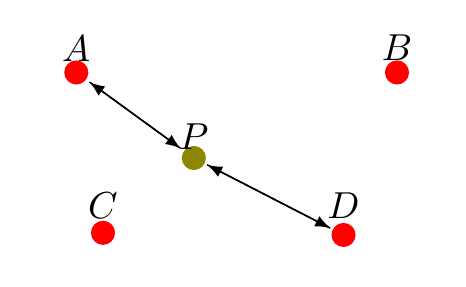
\includegraphics[width=.75\textwidth]{figures/triangle}
 \caption[Closest Directions ] {
 	{\bf Closest Directions}

	}
 \label{fig:triangle}
\end{figure} 

We, then reduce to the three closest directions, so less interpolation weights are to be computed.

One possible way to find the closest three directions is to compute the distance between $P$ and all other four directions and to discard the furthest one.
However, this is computational heavy for real-time applications.
The less computational demanding way is to approximately find triangle to which $P$ belongs, i.e. $ABC$ or $CBD$.
The following method produces unnoticeable differences of visual results compared to the method which tests if the point $P$ belongs to $ABC$ or $CBD$.


We compute to which direction $P$ is closer, i.e. whether to $A$ or $D$. The distance is computed as follows:

{\centering$d=\sqrt{(x-x^{'})^2+(y-y^{'})^2+(z-z^{'})^2}=
\sqrt{r^2+r^{'2}-2rr'({\color{blue} sin(\theta)sin(\theta^{'})}{\color{magenta}cos(\phi)cos(\phi^{'})}+{\color{blue} sin(\theta)sin(\theta^{'})}{\color{magenta} sin(\phi)sin(\phi^{'})}+cos(\theta)cos(\theta^{'}))}=
\sqrt{r^2+r^{'2}-2rr'({\color{blue} sin(\theta)sin(\theta^{'})}{\color{magenta}cos(\phi-\phi^{'})}+cos(\theta)cos(\theta^{'}))}$\\}


Note that, in practice $r$ and $r^{'}$ are equal 1. As we are interested in comparing distances it is enough to compare this term: 

{\centering$d^{'}=sin(\theta)sin(\theta^{'})cos(\phi-\phi^{'})+cos(\theta)cos(\theta^{'})$\\}

The bigger the term  $d^{'}$ the smaller the overall distance, because there is negative sign in the formula $d$. 
If $P$ is closer to $A$, the resulting three directions are $A$, $B$, $C$.
If $P$ closer to $D$ then $B$, $C$, $D$.

If the input direction $P$ is beyond the measuring directions, i.e. $\theta_p>\Delta \theta*n$ for any $n$.
We take the two closer measured directions, i.e.  $C=(\theta_{U},\phi_{L}^2)$ and $D=(\theta_{U},\phi_{U}^2)$ and perform linear interpolation between these two directions.


\subsection{Barycentric Coordinates}
\label{chapter:barycentric}
A common interpolation technique for the BTF is barycentric coordinates interpolation. 
However, as it is computational heavy, the approximation algorithm proposed by Hatka and Haindl \cite{btfblender} will be used.

Assume that a triangle $P_{1}P_{2}P_{3}$ bounds input point P, for which we want to compute interpolation weights. 
Figure \ref{fig:acquisition_example} demonstrates the hemisphere on which triangle $P_{1}P_{2}P_{3}$ lies.
$C_{P}$ denotes desired pixel color. 
In general, linear interpolation of that pixel will be $C_{P}=w_{1}C_{P1} + w_{2}C_{P2} + w_{1}C_{P2}$, 
where $C_{P1},C_{P2},C_{P3}$ correspond to color values of the found triangle $P_{1}P_{2}P_{3}$. Weights $w_{1},w_{2},w_{3}$ are normalized and sum up to $1$.

Weights  $w_{1},w_{2},w_{3}$ defined as volumes $V_{1},V_{2},V_{3}$ which correspond to $PP_{2}P_{3}O$, $PP_{3}P_{1}O$, $PP_{1}P_{2}O$ tetrahedrons, where $O=(0,0,0)$.
 Volumes calculated as determinates of $4\times 4$ matrices

{\centering $w_{1}:=V_{1}=\frac{1}{6}\left | det(PP_{2}P_{3}O) \right |$ \\}
{\centering $w_{2}:=V_{2}=\frac{1}{6}\left | det(PP_{3}P_{1}O) \right |$ \\}
{\centering $w_{3}:=V_{3}=\frac{1}{6}\left | det(PP_{1}P_{2}O) \right |$ \\}

Last step is the normalization of found volumes, i.e. $V_{i}=\frac{V_{i}}{\sum_{i=1}^{3}V_{i}}$.


\subsection{Algorithm}
\label{chapter:interp_algo}

Computing interpolation weights for input direction $P$, it is required to find the closest measured directions $P_{1}P_{2}P_{3}$ to $P$.
After these three directions are known for the input direction $P$, interpolation weights can be computed.
 Chapter \ref{chapter:barycentric} explains how to compute barycentric coordinates, i.e interpolation weights.
  
To compute the final interpolated color we combine interpolation weights of light and camera directions.
Assume that $I$ and $O$ are input light and camera directions. 
Then, bounding triangles for both of them are $I_{1}I_{2}I_{3}$ and $O_{1}O_{2}O_{3}$ accordingly.
Corresponding barycentric weights then are $b_{i}=[b_{i1},b_{i2},b_{i3}]^T$ and $b_{o}=[b_{o1},b_{o2},b_{o3}]^T$.
The final color is the linear combination of $b_{i}$, $b_{o}$ weights and known measured color values 

 {\centering $ C_{f}=\sum_{u=1}^{3}b_{iu}\sum_{v=1}^{3}b_{ov}C_{uv},$\\} where $C_{uv}$ is a color value that corresponds for a light direction $I_{u}$ and a camera direction $O_{v}$.

